\documentclass[tikz,border=4pt]{standalone}
\usepackage{amsmath}
\begin{document}
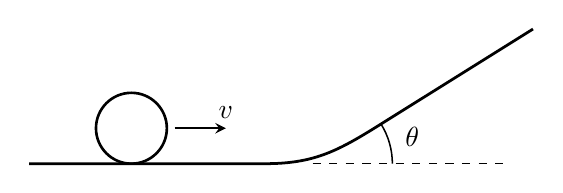
\begin{tikzpicture}[>=stealth, thick, scale=1.0]
  % Horizontal floor curving smoothly into incline of angle theta = 32 deg
  \draw[line width=1.0pt] (0, 0) -- (3.0, 0)
    .. controls (3.6, 0) and (3.9, 0.15) .. (4.4, 0.46)
    -- (6.4, {0.46 + 2.0*tan(32)});

  % Horizontal reference dashed line for incline angle theta
  \draw[dashed, line width=0.55pt] (3.6, 0) -- (6.1, 0);

  % Sphere rolling on flat surface
  \draw[line width=0.95pt] (1.3, 0.45) circle (0.45);
  \draw[->, line width=0.7pt] (1.85, 0.45) -- (2.5, 0.45) node[above] {$v$};

  % Angle theta arc (intersection of incline line with y=0: x_int = 4.4 - 0.46/tan(32) = 3.664)
  \draw[line width=0.55pt] (3.664, 0) ++(0:0.95) arc[start angle=0, end angle=32, radius=0.95];
  \node at ({3.664 + 1.25*cos(16)}, {1.25*sin(16)}) {$\theta$};
\end{tikzpicture}
\end{document}
